\subsubsection{UC7 - Selezione lingua}\label{UC7}

\begin{figure}[H]
  \centering
  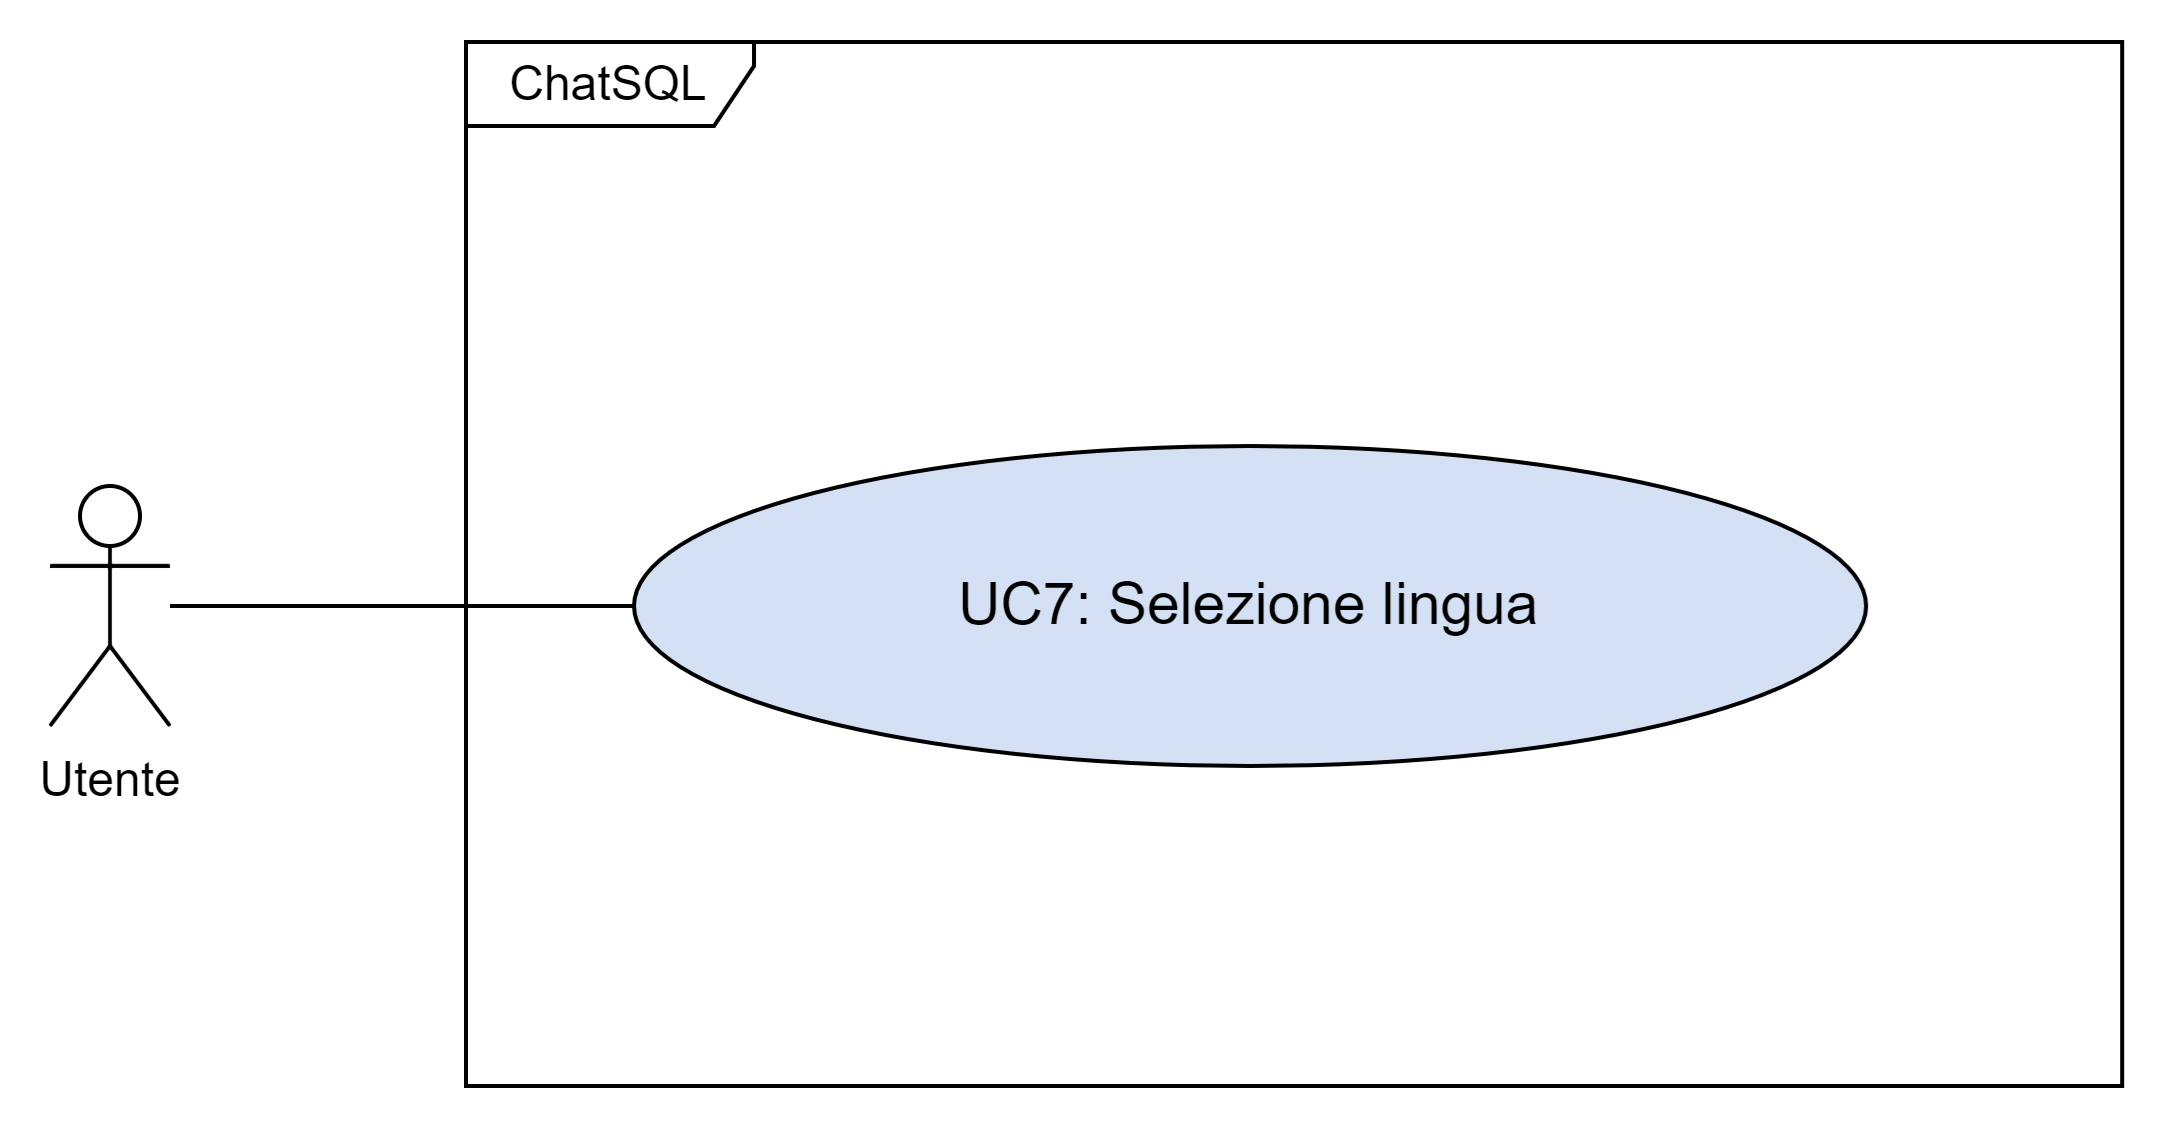
\includegraphics[width=0.90\textwidth]{assets/uc7.png}
  \caption{UC7}
\end{figure}

\paragraph*{Descrizione}
L'Utente seleziona una lingua con cui effettuare la richiesta al ChatBOT. 

\paragraph*{Attori principali}
Utente

\paragraph*{Precondizioni}
\begin{itemize}
  \item L'applicazione è stata avviata con successo;
  \item L'Utente sta visualizzando correttamente la chat.
\end{itemize}

\paragraph*{Postcondizioni}
\begin{itemize}
  \item L'Utente ha selezionato una lingua tra quelle disponibili.
\end{itemize}

\paragraph*{Trigger}
L'Utente vuole selezionare una lingua per la generazione del \glossario{prompt}.

\paragraph*{Scenario principale}
\begin{enumerate}
  \item L'Utente seleziona una lingua da una lista predefinita. La scelta è tra le seguenti lingue:
    \begin{itemize}
      \item Inglese;
      \item Italiano;
      \item Francese;
      \item Spagnolo;
      \item Tedesco.
    \end{itemize}
\end{enumerate}

% TODO [in caso di errore ed incongruenza tra la lingua scritta e quella selezionata teniamo solo errore uc6 del \glossario{prompt}? O viene controllata prima?]
